% Manuscrito MICAI 2027. Compilar con:  pdflatex main && bibtex main && pdflatex main && pdflatex main
% Version anonima para revision:  \anontrue  (por defecto).  Camera-ready: \anonfalse
\documentclass[runningheads]{llncs}

% Compilacion reproducible: sin estos tres, pdflatex incrusta la fecha y un identificador
% aleatorio en cada corrida, y el MD5 del PDF de envio cambia sin que cambie una sola palabra.
\pdfinfoomitdate=1
\pdftrailerid{}
\pdfsuppressptexinfo=-1

\newif\ifanon
\anontrue

\usepackage{cmap}
\usepackage[T1]{fontenc}
\usepackage[utf8]{inputenc}
\usepackage{graphicx}
\usepackage{booktabs}
\usepackage{amsmath}
\usepackage{amssymb}
\usepackage{siunitx}
\usepackage{xurl}
\usepackage[hidelinks]{hyperref}

\sisetup{group-minimum-digits=4, detect-weight=true, detect-family=true}
\graphicspath{{figures/}}
\emergencystretch=1em
\AtBeginDocument{\pdfpagewidth=210mm \pdfpageheight=297mm}

\begin{document}

\title{How Much of That Gain Is the Denominator?\texorpdfstring{\\}{ }A Control for Legend Shrinking in Imbalanced Crop Mapping}
\titlerunning{How Much of That Gain Is the Denominator?}

\ifanon
  \author{Anonymous Author(s)}
  \institute{Anonymous Institution}
\else
  \author{Arthur Zizumbo\inst{1} \and Javier A. Rebull-Saucedo\inst{1}\thanks{Corresponding author.}}
  \institute{Anonymous Institution, City, Country\\
    \email{author@example.org}}
\fi

\maketitle

\begin{abstract}
Parcel-level crop maps are routinely evaluated with macro-averaged F1 over a catalog of classes the
practitioner has already pruned, and the pruning is reported, when it is reported at all, as a
property of the data rather than as a decision. We ask how much of the resulting gain belongs to
the mechanism that pruned the catalog and how much to the smaller denominator that pruning
creates. We formalize two operating mechanisms that trade coverage for macro quality, shrinking the
promised legend and abstaining on low-confidence parcels, and evaluate them under a spatial-block
protocol that chooses the operating point outside the data used to measure it, scores both
mechanisms over the same class set, and never consults a label to decide what to deliver. Against a
control that scores the untouched predictor over the same shrunken legend while delivering
everything, most of the apparent gain disappears: on a first public benchmark the control accounts
for most of it, on a second benchmark in a different year and region for almost all of it, and over
the range where coverage stays complete for the entire gain, with every mechanism returning
identical numbers. At matched coverage, abstention outperforms legend shrinking on both benchmarks,
and retiring classes by low support, which is what practitioners report doing, is the weakest
criterion we test and is not monotone in the number of classes retired. A macro-averaged figure
computed over a pruned catalog is therefore uninterpretable without this control, which costs one
line to compute.

\keywords{Crop mapping \and Class imbalance \and Selective classification \and Evaluation
protocol \and Spatial cross-validation}
\end{abstract}

\section{Introduction}
\label{sec:introduction}

A parcel-level crop map promises a catalog. The catalog is a decision: someone chose which crop
types the product will name and which it will not, and that choice is made long before any
accuracy figure is computed. In practice the choice is rarely reported as a choice. It arrives in a
sentence about how some classes had too few samples, and the evaluation that follows is computed
over whatever survived.

This matters because the metric that dominates the literature on imbalanced crop mapping is
macro-averaged F1, and macro-averaging divides by the number of classes. Removing a class the model
handled badly raises the macro average twice over: once by deleting a low per-class score from the
numerator, and once by shrinking the denominator. The second effect requires no model, no
mechanism, and no work. It is arithmetic. Yet a gain produced entirely by the second effect is
indistinguishable, in a results table, from a gain produced by a method.

We take that ambiguity as the object of study. We consider two mechanisms that a practitioner can
use to trade coverage for macro quality. The first shrinks the promised legend: the product names
$K$ of the $C$ available classes and declines to answer wherever its unrestricted prediction falls
outside them. The second keeps the full legend and abstains on the parcels where the predictor is
least confident, in the tradition of selective classification
\cite{chow1970reject,geifman2017selective}. Both reduce how much of the map is delivered; both
raise the macro figure;
and the question is how much of that rise either one is responsible for.

Our answer is a control, and it is almost embarrassingly cheap. Score the \emph{untouched}
predictor over the same shrunken legend while delivering everything. Whatever that control
recovers was never bought by the mechanism. On a first public benchmark of eighteen agronomic
classes, the control accounts for \num{88.3}\,\% of the apparent gain from shrinking the catalog
from eighteen classes to eight. On a second benchmark, in a different year, a different region and
with a different model family, it accounts for \num{95.1}\,\% at the pre-registered operating
point. And over the range where coverage remains complete, it accounts for \emph{all} of it: every
mechanism we test returns the same number, to four decimals, while the macro figure climbs by
\num{0.2447}.

Two further results follow from the same protocol. At matched coverage, abstaining on
low-confidence parcels outperforms shrinking the legend on both benchmarks, which is the opposite
of what the practice we set out to formalize assumes. And retiring classes by low support, which is
the criterion practitioners describe using, is the weakest of the three we test and is not monotone
in the number of classes retired: retiring more can make the delivered map worse.

The contributions are as follows. We formalize the two mechanisms and give a spatial-block protocol
that chooses the operating point outside the data used to measure it, scores both mechanisms over
the same class set so that their numbers are comparable, and never consults a ground-truth label to
decide which parcels to deliver. We quantify the decomposition of the apparent gain into
denominator and mechanism on two public benchmarks under an unchanged protocol. We order the three
retirement criteria with paired bootstrap intervals and a multiplicity correction. And we show that
a trained stacking meta-learner performs the same retirement implicitly and undeclared, and that
the difference between measuring it inside and outside the sample is enough to reverse the
conclusion about whether the ensemble helps at all.

\section{Related Work}
\label{sec:related}

We organize related work by what each line of research establishes and where it stops, because the
gap this paper addresses lies in the space between two literatures that rarely meet.

\paragraph{Selective classification.}
The option to abstain is old and well characterized. Chow's rule fixes the optimal
error--reject tradeoff for a known posterior \cite{chow1970reject}, and the modern treatment
extends it to deep networks with learned or calibrated rejection
\cite{geifman2017selective,geifman2019selectivenet,liu2019deepgamblers}, with recent surveys
mapping the design space \cite{hendrickx2024rejectsurvey,hasan2023uncertaintysurvey}. Two
refinements matter here: the observation that a single risk--coverage curve hides which groups pay
for the abstention \cite{jones2020selectivedisparities}, and the extension of reject curves to
precision and recall rather than error alone \cite{fischer2023rejectcurves,pugnana2022aucselective}.
What this literature does not treat is abstention by \emph{class}: its unit of rejection is the
sample, so a mechanism that declines to name an entire category falls outside its formalism, and
the interaction between that mechanism and a macro-averaged metric is not analyzed.

\paragraph{Class structure in crop mapping.}
Work on crop mapping does manipulate the class catalog, but as a modeling device rather than as an
operating point. Turkoglu et al.\ organize crop types into a hierarchy and let the model back off
to a coarser level when the fine-grained decision is unreliable \cite{turkoglu2021hierarchies},
which is the closest existing mechanism to legend shrinking; the evaluation, however, reports
overall accuracy on a single split, so the effect on a macro average and its variability across
space are not measured. Pan-European harmonization efforts confront the same problem at the level
of the nomenclature itself \cite{schneider2021eurocrops,claverie2026eurocropsv2}, and fine-grained
mapping work notes the cost of rare classes without isolating it
\cite{lei2025finecrop,li2021costeffective,donmez2025cropcover}. Across this literature the pruned
catalog is reported as a property of the data.

\paragraph{Benchmarks and temporal models.}
We evaluate on two public parcel-level benchmarks. PASTIS provides Sentinel-2 time series with
panoptic annotations over France \cite{garnot2021pastis}; BreizhCrops provides a larger parcel-level
collection over Brittany with a native partition by administrative region and an extreme class
distribution \cite{russwurm2020breizhcrops}. The temporal architectures we use as predictors are
standard: temporal convolutions \cite{pelletier2019tempcnn}, self-attention over raw series
\cite{russwurm2020selfattention}, and vision transformers adapted to satellite image time series
\cite{tarasiou2023tsvit}. None of these are contributions of this paper; they supply the posteriors
over which the protocol operates.

\paragraph{Evaluation protocol.}
That the protocol is spatial rather than random is not optional. Cross-validation that ignores
spatial autocorrelation inflates estimates of predictive performance, sometimes severely
\cite{roberts2017crossvalidation,ploton2020spatialvalidation}. We therefore choose every operating
point on spatial blocks disjoint from the block it is evaluated on. The ensembling literature
supplies the remaining ingredient, the stacking meta-learner whose implicit behavior we examine
\cite{wolpert1992stacking,zhang2022ensemblereview,abdali2023parallelcascaded}, and it is precisely
Wolpert's requirement of leakage-free partitions for training the second-level model that our
in-sample versus out-of-sample comparison puts to the test.

\section{Materials and Method}
\label{sec:method}

\subsection{Data}
\label{sec:data}

We use two public parcel-level benchmarks and never tune the protocol between them.

\begin{figure}[tbp]
\centering
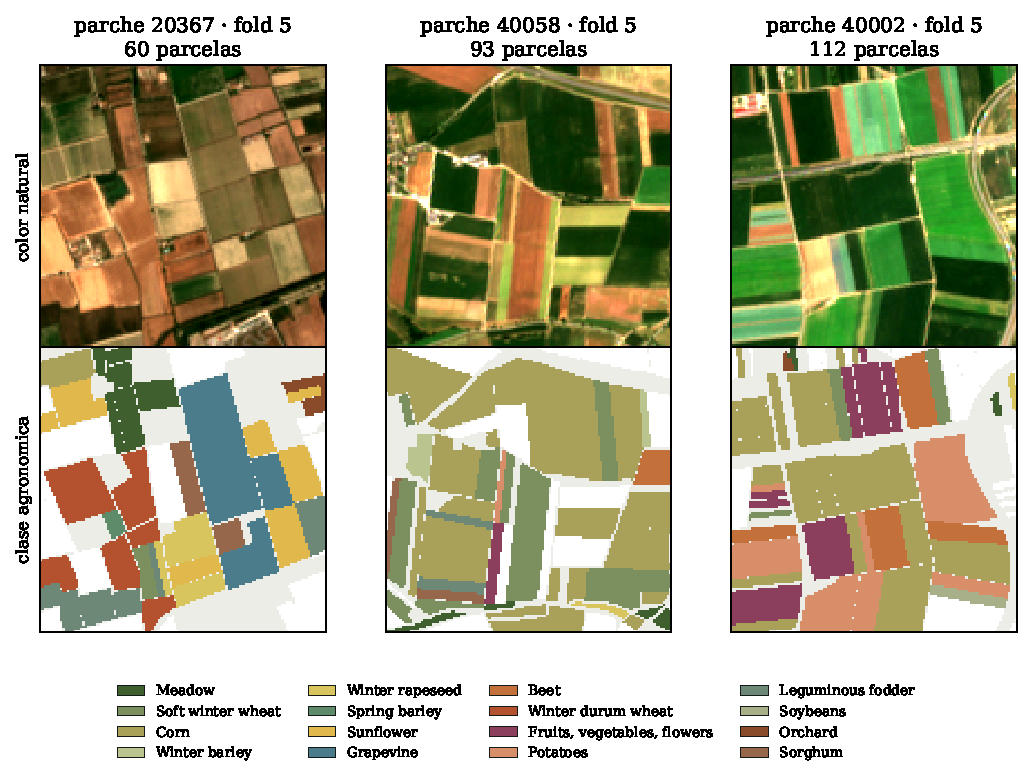
\includegraphics[width=\textwidth]{parcelas.pdf}
\caption{Three patches of the held-out fold of the primary benchmark. Top: natural-color
Sentinel-2 composite from the acquisition nearest to 1 July. Bottom: the parcel-level agronomic
annotation. The unit of the product is the parcel, and the catalog this paper studies is the list
of names the bottom row is allowed to use.}
\label{fig:patches}
\end{figure}

\begin{table}[tbp]
\caption{The two benchmarks. Both are described by the same \num{185}-dimensional temporal
feature vector, so the replication varies data, year, region and model family, but not
representation.}
\label{tab:benchmarks}
\centering
\begin{tabular}{lrr}
\toprule
 & primary (PASTIS) & replication (BreizhCrops) \\
\midrule
Season & 2018--2019 & 2017 \\
Region & metropolitan France & Brittany \\
Parcels scored & 16\,640 & 60\,000 \\
Classes & 18 & 9 \\
Majority class & 6\,128 & 18\,113 \\
Minority class & 103 & 2 \\
Imbalance ratio & 60:1 & 9\,057:1 \\
Blocks & 5 spatial (H3, 1\,km buffer) & 2 administrative regions \\
Predictor & pre-trained members & gradient boosting, leave-one-region-out \\
\bottomrule
\end{tabular}
\end{table}

The \textbf{primary benchmark} is PASTIS \cite{garnot2021pastis}. We obtain it through the
PASTIS-R distribution, which adds aligned radar series \cite{saintefaregarnot2022multimodal}, but
\emph{we use its optical modality only}: every predictor here reads Sentinel-2, so calling the
benchmark PASTIS-R would name a sensor we never touch. From it we take the
held-out fold and aggregate the dense annotations to parcel level, yielding \num{16640} parcels
across \num{496} image patches and eighteen agronomic classes. Its imbalance is severe: the
majority class holds \num{6128} parcels and the minority class \num{103}, a ratio of roughly
\num{60}:\num{1}.

The \textbf{replication benchmark} is BreizhCrops \cite{russwurm2020breizhcrops}, Sentinel-2 L2A
series over Brittany for the 2017 season, with nine agronomic classes and a native partition into
administrative regions. We use regions \texttt{frh01} and \texttt{frh04} with a proportional
stratified subsample of \num{30000} parcels each, fixed seed, for a total of \num{60000} parcels.
Its imbalance is an order of magnitude worse than the primary benchmark: in the full index the
majority class outnumbers the minority by up to \num{19207}:\num{1}, and in our subsample three of
the nine classes hold two, seven and \num{289} parcels respectively. Both benchmarks are described
by the same \num{185}-dimensional temporal feature vector, derived from seventeen spectral indices,
so that the two experiments differ in data and model but not in representation.

\begin{figure}[tbp]
\centering
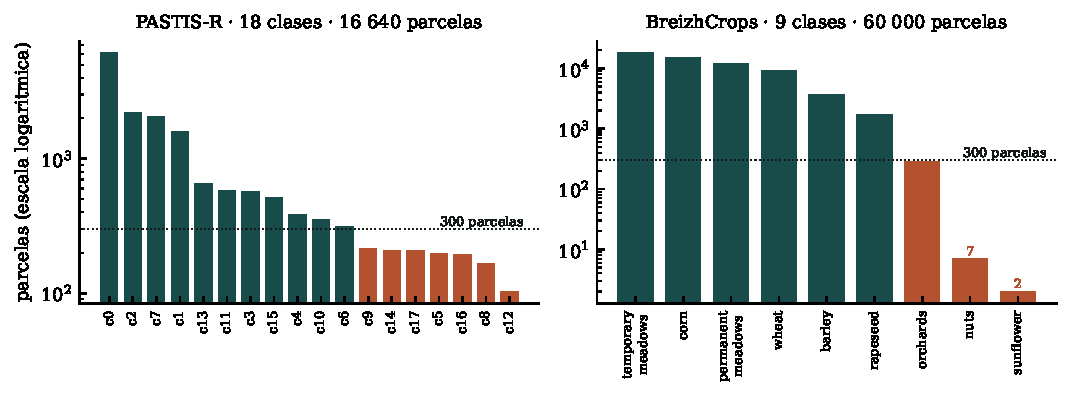
\includegraphics[width=\textwidth]{soporte.pdf}
\caption{Class support on a logarithmic scale. Bars below \num{300} parcels are drawn in the
accent color: these are the classes every retirement criterion removes first. The replication
benchmark's tail is not merely thinner, it is degenerate --- two and seven parcels --- which is
what makes the corridor of Sect.~\ref{sec:corridor} possible.}
\label{fig:support}
\end{figure}

\subsection{Predictors}
\label{sec:predictors}

The protocol operates on posteriors and is agnostic to how they were produced. On the primary
benchmark we take the two strongest of ten available members, a vision transformer for satellite
image time series \cite{tarasiou2023tsvit} and a gradient-boosted model over learned embeddings.
On the replication benchmark we train a gradient-boosted classifier \emph{leaving one region out}:
each parcel's posterior comes from a model that never saw its region, which makes every posterior
we score a genuine out-of-region prediction. That classifier reaches macro-F1 \num{0.4979} and
accuracy \num{0.7421} on \texttt{frh01}, and \num{0.4811} and \num{0.7257} on \texttt{frh04}.

\subsection{Blocks}
\label{sec:blocks}

Every operating point is chosen on data disjoint from the data that measures it. On the primary
benchmark the blocks are spatial: an H3 tessellation at resolution five, clustered and separated by
a \SI{1}{\kilo\meter} buffer, giving five blocks. On the replication benchmark the index publishes
no per-parcel coordinates, so the finest spatial structure available is the administrative region;
we use the two regions as the two blocks. This is a real limitation and we treat it as one: with
two blocks the resampling captures variation \emph{within} regions and not \emph{between} them, so
we report the per-block difference for every contrast rather than a pooled interval alone.

\subsection{The two mechanisms, and a third criterion}
\label{sec:mechanisms}

Let $\mathcal{C}$ be the full set of $C$ classes, $p(\cdot \mid x)$ the predictor's posterior for
parcel $x$, and $\hat{y}(x) = \arg\max_{c \in \mathcal{C}} p(c \mid x)$ its unrestricted
prediction.

\emph{Legend shrinking} selects a subset $\mathcal{L} \subseteq \mathcal{C}$ with
$|\mathcal{L}| = K$ on the training blocks, and on the evaluation block delivers a parcel when
$\hat{y}(x) \in \mathcal{L}$, emitting $\arg\max_{c \in \mathcal{L}} p(c \mid x)$. We test two
criteria for choosing $\mathcal{L}$: by per-class F1 on the training blocks, and by class support
on the training blocks, the latter because it is what practitioners report doing.

\emph{Confidence rejection} keeps $\mathcal{L} = \mathcal{C}$ and delivers the parcels whose
$\max_c p(c \mid x)$ falls above a threshold. The threshold is the quantile of the block's own
confidences that matches the number of parcels the comparison mechanism delivered in that same
block, so the two are compared at equal coverage.

Neither mechanism reads a ground-truth label to decide what to deliver. This is worth stating
explicitly because the natural implementation of legend shrinking does read one: delivering the
parcels whose \emph{true} label lies in $\mathcal{L}$ is an oracle, and it inflates the mechanism's
apparent quality. Our delivery rule uses the unrestricted argmax, which is observable at inference
time.

\subsection{The aligned estimand}
\label{sec:estimand}

Two mechanisms that promise different catalogs cannot be compared by each one's own macro average,
because the averages are taken over different denominators. We therefore score every mechanism with

\begin{equation}
  \mathrm{F1}_{\text{aligned}} \;=\; \frac{1}{|\mathcal{L} \cap \mathcal{Y}|}
  \sum_{c \,\in\, \mathcal{L} \cap \mathcal{Y}} \mathrm{F1}_c ,
  \label{eq:aligned}
\end{equation}

\noindent where $\mathcal{L}$ is the legend under test and $\mathcal{Y}$ the classes actually
present among the delivered parcels. Both mechanisms in a contrast are scored over the \emph{same}
$\mathcal{L}$. We also report each mechanism's native macro over what it individually promises, but
only as a product-facing view; it is not comparable across mechanisms and we never use it for a
contrast.

\subsection{The control}
\label{sec:control}

The control that gives this paper its title is one line. For each legend $\mathcal{L}$ and each
block, score the untouched predictor over $\mathcal{L}$ using Eq.~\ref{eq:aligned} while delivering
\emph{every} parcel. No class is retired from the emission, no parcel is refused; only the
denominator changes. If this control matches or exceeds a mechanism, the quality was bought by the
choice of class set and not by the mechanism.

\subsection{Inference}
\label{sec:inference}

Contrasts use a paired bootstrap: one resample index is drawn per block and \emph{both} mechanisms
are rescored on it, so the two share the sampling noise. We draw \num{1000} resamples and report
the percentile interval of the difference of mean block-level aligned F1, together with the
per-block differences. On the primary benchmark we additionally resample by image patch rather
than by parcel, since parcels within a patch share an image and are not independent. The
pre-registered principal criterion is $K = \lceil C/2 \rceil$; the remaining values of $K$ form an
exploratory family, corrected by the Holm--Bonferroni step-down procedure within each predictor and
each benchmark.

\section{Results}
\label{sec:results}

\subsection{The corridor where every mechanism is identical}
\label{sec:corridor}

On the replication benchmark, shrinking the catalog from nine classes to six raises aligned macro
F1 from \num{0.4895} to \num{0.7342}, an apparent gain of \num{0.2447}. Over that entire range all
four series --- retirement by F1, retirement by support, confidence rejection, and the control that
applies no mechanism at all --- return the \emph{same} value, and coverage stays at
\num{1.000}.

The reason is arithmetic and it is what makes the observation conclusive. The three classes
retired first hold two, seven and \num{289} parcels out of \num{60000}; the unrestricted argmax
essentially never predicts them, so removing them from the legend removes no parcel from the
delivered map. No mechanism does anything. The metric rises by almost a quarter of a point on its
own.

\begin{table}[tbp]
\caption{Decomposition of the apparent gain on the replication benchmark, nine-class universe.
``Denominator'' is the control of Sect.~\ref{sec:control}: the untouched predictor scored over the
same legend, delivering everything. $K = 5$ is the pre-registered principal criterion.}
\label{tab:decomposition}
\centering
\begin{tabular}{rrrrrr}
\toprule
$K$ & aligned F1 & apparent gain & denominator & mechanism & coverage \\
\midrule
9 & 0.4895 & ---     & ---              & ---            & 1.000 \\
8 & 0.5507 & +0.0612 & +0.0612 (100.0\%) & +0.0000 (0.0\%) & 1.000 \\
7 & 0.6293 & +0.1398 & +0.1398 (100.0\%) & +0.0000 (0.0\%) & 1.000 \\
6 & 0.7342 & +0.2447 & +0.2447 (100.0\%) & +0.0000 (0.0\%) & 1.000 \\
\textbf{5} & \textbf{0.8055} & \textbf{+0.3160} & \textbf{+0.3004 (95.1\%)} & \textbf{+0.0156 (4.9\%)} & \textbf{0.859} \\
4 & 0.8579 & +0.3684 & +0.3352 (91.0\%) & +0.0333 (9.0\%) & 0.806 \\
3 & 0.9126 & +0.4232 & +0.3826 (90.4\%) & +0.0406 (9.6\%) & 0.444 \\
\bottomrule
\end{tabular}
\end{table}

\subsection{The decomposition transports}
\label{sec:transport}

The same protocol, unchanged, gives the same qualitative answer on the primary benchmark. Shrinking
from eighteen classes to eight raises aligned macro F1 from \num{0.5612} to \num{0.8052}, an
apparent gain of \num{0.2440}, of which the control recovers \num{0.2155}, or
\num{88.3}\,\%. At the pre-registered operating point of $K = 9$ the control recovers
\num{87.1}\,\% and the result holds for both of the two predictors we tested.

Two benchmarks, two years, two regions, two model families and one protocol therefore agree: the
denominator dominates. Where they differ is in degree, and in the direction that matters for a
practitioner: the replication benchmark, whose imbalance is an order of magnitude worse, leaves the
mechanism even less to explain.

\begin{figure}[tbp]
\centering
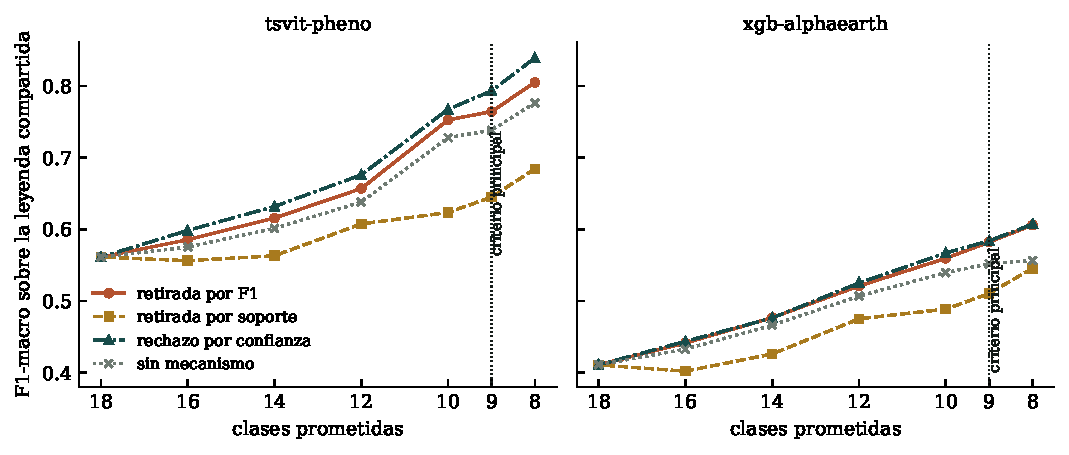
\includegraphics[width=\textwidth]{frontier-primary.pdf}
\caption{The same frontier on the primary benchmark, for its two strongest predictors. The control
that applies no mechanism (crosses) already recovers most of the distance travelled by the
mechanisms, and retirement by support (squares) again trails the other two throughout.}
\label{fig:primary}
\end{figure}

\begin{figure}[tbp]
\centering
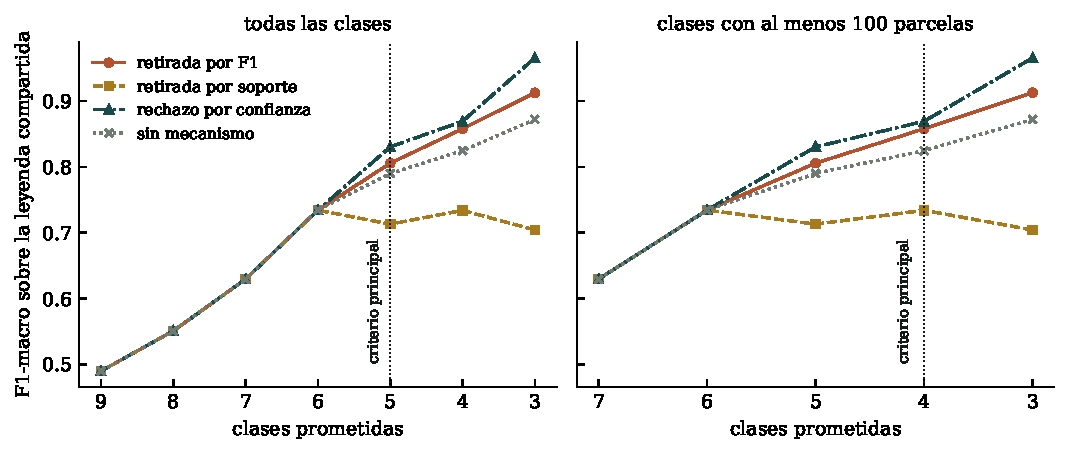
\includegraphics[width=\textwidth]{frontier-replication.pdf}
\caption{Quality--coverage frontier on the replication benchmark, in the two pre-registered class
universes. The four series are indistinguishable until $K = 6$ because coverage is complete and no
mechanism acts; the dotted line marks the principal criterion. Retirement by support (squares) is
the only series that falls as more classes are retired.}
\label{fig:replication}
\end{figure}

\subsection{At equal coverage, abstention wins}
\label{sec:ordering}

Once coverage falls below one and the mechanisms begin to differ, they can be ordered. At the
principal criterion of the replication benchmark, confidence rejection reaches \num{0.8303} against
\num{0.8055} for legend shrinking at the same coverage, a difference of \num{-0.0248} with a paired
\num{95}\,\% interval of $(-0.0272, -0.0225)$ and a Holm-adjusted $p$ below \num{0.0001}. Both
regions agree in sign and magnitude, at \num{-0.0248} and \num{-0.0249}.

On the primary benchmark the difference has the same sign but is not distinguishable from zero:
\num{-0.0288} with an interval of $(-0.0414, +0.0080)$ and a Holm-adjusted $p$ of \num{0.336}. The
honest summary across both benchmarks is therefore that we find no evidence that shrinking the
legend outperforms abstention, and on the larger and more imbalanced benchmark we find significant
evidence of the reverse.

\begin{figure}[tbp]
\centering
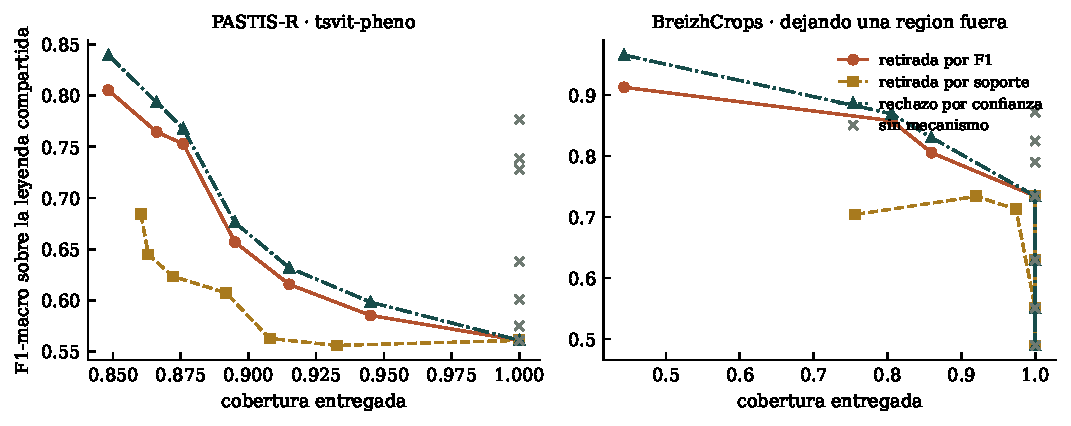
\includegraphics[width=\textwidth]{cobertura.pdf}
\caption{The same measurements plotted against delivered coverage rather than legend size, which
is how the selective classification literature reads them. The control (crosses) sits on the
coverage-one vertical by construction, since it never withholds anything; the point of the figure
is how many of those crosses lie \emph{above} the mechanisms' curves at lower coverage.}
\label{fig:coverage}
\end{figure}

\subsection{Retirement by support is the weakest criterion, and it is not monotone}
\label{sec:support}

Retiring classes by low support is the criterion practitioners describe using, and it is the worst
of the three on both benchmarks. On the replication benchmark it reaches \num{0.7129} at the
principal criterion against \num{0.8055} for retirement by F1, a gap of \num{0.0926}, which widens
to \num{0.2085} at $K = 3$. On the primary benchmark the corresponding gap is between \num{0.12}
and \num{0.13}.

It also does something neither other criterion does: it \emph{degrades} as more classes are
retired, from \num{0.7129} at $K = 5$ to \num{0.7041} at $K = 3$. Inspecting the legends explains
why. Support-based retirement removes rapeseed, which holds \num{1718} parcels and which the model
separates well, while retaining both meadow classes, which the model confuses with each other. The
criterion optimizes sample size, which is not the same quantity as the quality of what is
delivered. Fig.~\ref{fig:legends} shows the substitution directly.

\begin{figure}[tbp]
\centering
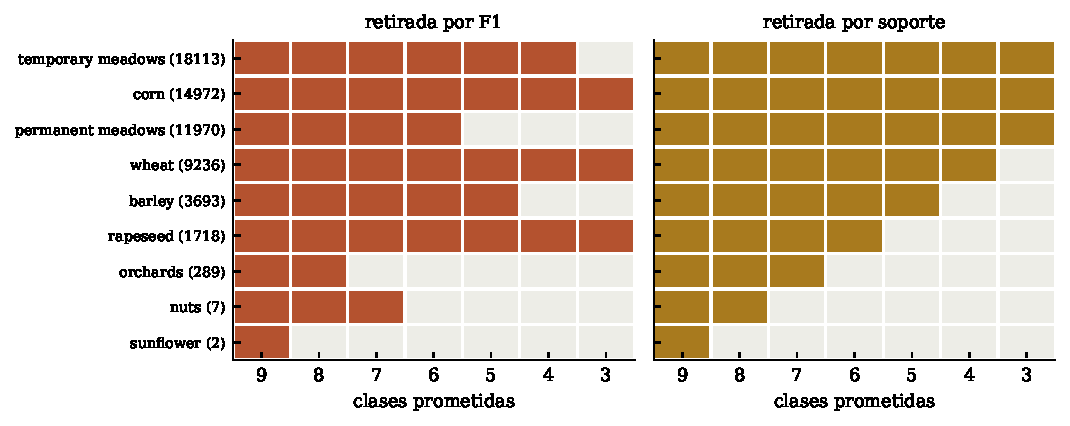
\includegraphics[width=\textwidth]{leyendas.pdf}
\caption{Which classes each criterion keeps as the legend shrinks, on the replication benchmark;
a filled cell means the class is promised. Support-based retirement (right) drops rapeseed at
$K = 5$ while keeping both meadow classes, which the model confuses with one another;
quality-based retirement (left) does the reverse. The two criteria disagree about exactly the
classes that decide the outcome.}
\label{fig:legends}
\end{figure}

\subsection{A trained meta-learner retires classes implicitly}
\label{sec:arbiter}

The mechanism this paper formalizes is already being applied, undeclared, by trained ensembles. On
the primary benchmark, a stacking meta-learner over three members drives one class of \num{355}
parcels to an F1 of exactly \num{0.0000}, while the best single model reaches \num{0.7790} on that
same class. The meta-learner has retired a class from the product without anyone choosing to, and
without it appearing anywhere in a results table.

\begin{table}[tbp]
\caption{Per-class F1 on the primary benchmark, leak-free, ordered by support. The trained
arbiter is the only combiner that zeroes a class, and it does so to one of \num{355} parcels that
every other combiner --- including the untrained mean --- handles above \num{0.77}. The retirement
is therefore a learned behavior, not a property of combining.}
\label{tab:perclass}
\centering
\small
\begin{tabular}{lrrrrr}
\toprule
Class & support & best single & mean & weighted vote & trained arbiter \\
\midrule
Meadow & 6\,128 & 0.9099 & 0.8980 & 0.9046 & 0.9138 \\
Corn & 2\,196 & 0.9295 & 0.8683 & 0.9053 & 0.9274 \\
Grapevine & 2\,067 & 0.9066 & 0.9141 & 0.9154 & 0.9124 \\
Soft winter wheat & 1\,584 & 0.8922 & 0.8466 & 0.8712 & 0.8886 \\
Leguminous fodder & 660 & 0.5087 & 0.3498 & 0.4707 & 0.5243 \\
Winter rapeseed & 387 & 0.9358 & 0.9153 & 0.9275 & 0.9377 \\
\textbf{Winter durum wheat} & \textbf{355} & \textbf{0.7790} & \textbf{0.7752} & \textbf{0.7782} & \textbf{0.0000} \\
Spring barley & 198 & 0.6667 & 0.4691 & 0.5879 & 0.5228 \\
Mixed cereal & 193 & 0.4949 & 0.3525 & 0.4302 & 0.2709 \\
Potatoes & 103 & 0.5595 & 0.5143 & 0.5638 & 0.5823 \\
\bottomrule
\end{tabular}
\end{table}

\begin{table}[tbp]
\caption{The same stacking meta-learner under three estimators. These are not three plausible
choices: the first is contaminated and the third is penalized by an aggregation artifact.}
\label{tab:regimes}
\centering
\begin{tabular}{lrl}
\toprule
Estimator & macro F1 & what it measures \\
\midrule
Refit on all parcels & 0.7470 & in-sample for the meta-learner \\
Pooled spatial out-of-fold & 0.6789 & leak-free, scored once \\
Mean of per-block macros & 0.5360 & leak-free, penalized by aggregation \\
\bottomrule
\end{tabular}
\end{table}

The regime in which such a meta-learner is measured is decisive. Scored in-sample --- refitted on
all parcels after cross-validation, which is the default of many stacking implementations --- it
reports \num{0.7470}. Scored leak-free by pooling its spatial out-of-fold posteriors and scoring
once, it reports \num{0.6789}. Averaging per-block macro scores instead of pooling reports
\num{0.5360}. The leakage accounts for \num{0.068} and the choice of aggregation for a further
\num{0.143}; conflating the two leads to reporting \num{0.536} as the honest figure when it is
\num{0.679}, penalizing the model for a measurement artifact on top of its actual error. Against
the best single model, the leak-free meta-learner loses by \num{0.0572} with an interval of
$(-0.0644, -0.0499)$ that excludes zero.

\section{Discussion}
\label{sec:discussion}

\paragraph{What each mechanism actually buys.}
Legend shrinking and confidence rejection both trade coverage for macro quality, but they charge
different customers. Shrinking the legend refuses an entire crop type everywhere: a farmer growing
it receives nothing, in every parcel, in every region. Abstention refuses individual parcels
scattered across all crop types, so no grower is systematically excluded, which is the selective
classification literature's own concern about who pays for the abstention
\cite{jones2020selectivedisparities}. Our measurements say that abstention is also the better buy
at equal coverage. The two arguments point the same way, and we know of no operational setting in
which the reverse is preferable except one: when the downstream consumer requires a fixed,
published catalog and cannot act on a partial map.

\paragraph{What should be reported.}
A macro-averaged figure computed over a pruned catalog is uninterpretable on its own, and the fix
is neither expensive nor novel. Report the number of classes the average is taken over, the
coverage the product delivers, and the control of Sect.~\ref{sec:control}. Three numbers, one of
which costs a single line of code. Without them, a paper that raises macro F1 by a quarter of a
point after retiring three rare classes is reporting arithmetic, and a reader cannot tell it from a
paper that improved a model.

\paragraph{On the criterion practitioners use.}
The finding that retirement by support is both the weakest criterion and non-monotone deserves
emphasis, because support is the criterion that gets used. It is chosen for a defensible reason ---
a class with few samples is a class whose estimate is unstable --- but instability of the estimate
and poor separability are different properties, and support only tracks the first. A class with
\num{1718} parcels that the model separates cleanly contributes more to a delivered map than two
abundant classes the model cannot tell apart. Choosing by measured per-class quality, on blocks
disjoint from those that will be evaluated, costs nothing extra and is strictly better in every
comparison we ran.

\paragraph{On measuring meta-learners.}
The three figures for the same stacking model --- \num{0.7470}, \num{0.6789} and \num{0.5360} ---
are not three plausible estimates to choose among. The first is contaminated, and Wolpert's
original formulation of stacking already required the leakage-free partitions it violates
\cite{wolpert1992stacking}. The third is leak-free but penalizes the model for an aggregation
artifact: averaging per-block macro scores in an imbalanced setting scores blocks over classes
their parcels do not contain. Pooling the out-of-fold posteriors and scoring once, which gives
\num{0.6789}, is the estimator that answers the question actually being asked. The gap between the
first and the last is wide enough to reverse a conclusion about whether the ensemble contributes
anything, which is why the regime has to be stated whenever such a number is printed.

\section{Limitations and Conclusion}
\label{sec:conclusion}

\paragraph{Limitations.}
Both benchmarks are French, so the replication varies year, region, class distribution and model
family, but not the agricultural system; whether the decomposition holds in a smallholder landscape
is open. On the replication benchmark the blocks are the two administrative regions, because the
published index carries no per-parcel coordinates, so our resampling captures variation within
regions and not between them; we report the per-block differences for this reason. That benchmark
also required imputing \num{1.62}\,\% of feature cells, concentrated in ratio indices whose
denominator involves a band the collection encodes as zero for masked pixels; the imputation uses
the training region's median only, and it cannot favor one mechanism over another because all
mechanisms read the same posterior. Finally, our out-of-fold posteriors on the primary benchmark
exist for a single fold, which is why the meta-learner of Sect.~\ref{sec:arbiter} is trained on
little data; that is a limitation of the artifacts available to us, not a claim about stacking in
general.

\paragraph{Conclusion.}
Macro-averaged F1 over a pruned class catalog mixes two things a reader cannot separate: what the
method did, and what the smaller denominator did. We gave a protocol that separates them, and the
answer on two public benchmarks is that the denominator dominates --- \num{88}\,\% on the first,
\num{95}\,\% on the second at the pre-registered operating point, and \num{100}\,\% over the range
where coverage stays complete and every mechanism returns an identical number. At equal coverage
we find no evidence that shrinking the legend beats abstaining, and significant evidence of the
reverse on the more imbalanced benchmark; the criterion practitioners report using, retirement by
low support, is the weakest we tested and degrades as more classes are retired. None of this
requires a new model. It requires reporting the class count, the coverage, and one control line
alongside every macro-averaged figure computed over a catalog someone chose.


\appendix
\section{Reproducibility}
\label{sec:appendix}

Every figure printed in this paper is re-derived from a file under version control whose MD5,
size and producing script are recorded in a custody ledger, and a gate recomputes those digests
and fails when any of them changes without being registered. The ledger currently holds
\num{62} sealed artifacts. The two benchmarks are public. The operating points, the class
universes and the principal criterion $K = \lceil C/2 \rceil$ were fixed in a written
pre-registration before the replication experiment was run; the two deviations forced by the data
--- the choice of blocks and the treatment of non-finite feature cells --- were written down as
dated amendments before any contrast was computed, together with the measurement error in our own
cost estimate that one of them corrected.


\bibliographystyle{splncs04}
\bibliography{refs}

\end{document}
